\section{Investigation of Genome Properties}
In order to gain a better understanding of the somewhat opaque GA process,
an experiment was designed with the goal of investigating the development of various properties of the population over time.

The "tricolor morphogenesis" was used as the basis for this experiment, since previous experiments with this problem showed it to be solvable, but not trivially simple for CA-NEAT.
The CA for this problem has $K=4$ cell states and the neighbourhood shape "Von Neumann" ($N=5$) was used.
An initial population of size $P=1000$ was created, with $N$ input nodes, $K$ output nodes and no initial hidden nodes.
This same population was then used as the initial population for five independent runs of $G=100$ generations, with different mechanisms of NEAT in use.
Table \ref{tbl:NEAT_incremental} shows which mechanisms are in use in which runs.

\begin{table}[h]
    \centering
    \caption{TODO}
    \begin{tabular}{c|ccccc}
    Run & Mutation & Crossover & Selection pressure & Speciation & Elitism \\ \hline
    A   & \checkmark        & ~         & ~                  & ~          & ~       \\
    B   & \checkmark        & \checkmark         & ~                  & ~          & ~       \\
    C   & \checkmark        & \checkmark         & \checkmark                  & ~          & ~       \\
    D   & \checkmark        & \checkmark         & \checkmark                  & \checkmark          & ~       \\
    E   & \checkmark        & \checkmark         & \checkmark                  & \checkmark          & \checkmark       \\
    \end{tabular}
    \label{tbl:NEAT_incremental}
\end{table}

Run A is a bit different, since it is not truly a GA run.
Instead the individuals that make up the population are mutated repeatedly, but crossover and elimination is not used.
Run B uses NEAT, however the selection is completely random, so there is no selection pressure.
Run C has selction pressure appropriate for the morphogenesis problem, but does not use the speciation mechanism of NEAT.
Run D is like C, but also uses the speciation mechanism.
And finally, run E uses all mechanisms of NEAT, including a pre-species elitism degree of $E=1$.

100 gens
    - only mutation
    - mutation + crossover, but fitness is constant
        -elitism=0
    - majority problem (do not stop scenario when f==1.0)
        -elitism=0?

investigate
    - lambda spread, mean, mode
    - genome size
    - change in enum-string
        - in terms of mean, median distance and bool(did change?)
    - amount of 'vestigial' nodes

\begin{figure}
\centering
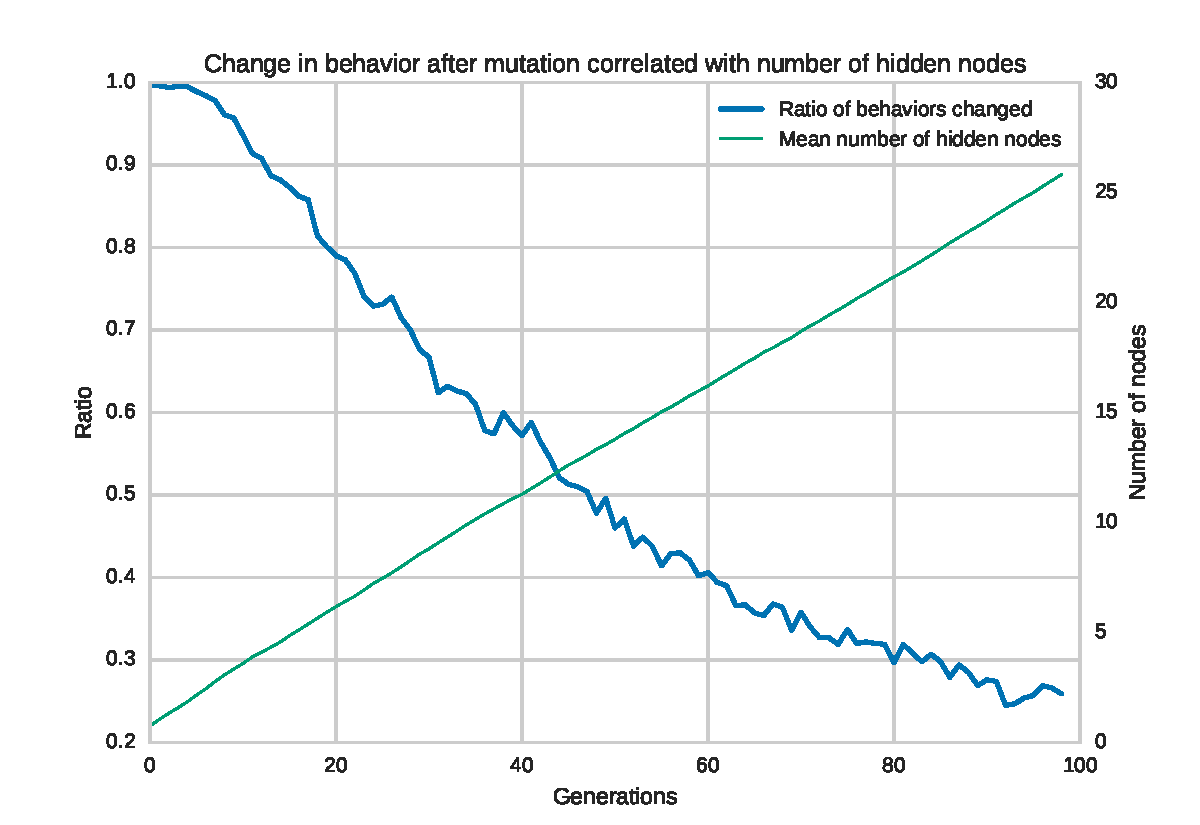
\includegraphics[width=\columnwidth]{fig/mutation_behavior_change}
\caption{TODO}
\end{figure}

\begin{figure}
\centering
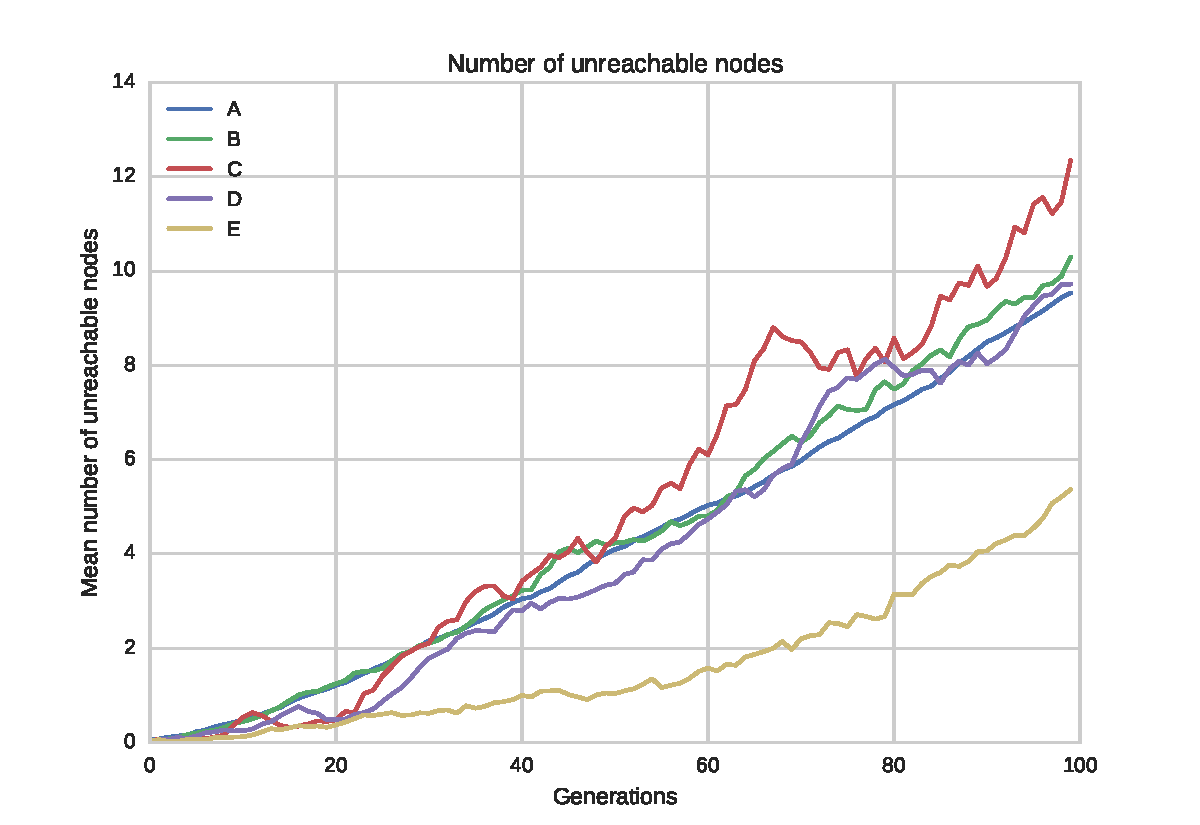
\includegraphics[width=\columnwidth]{fig/vestigial_nodes}
\caption{TODO}
\end{figure}

\begin{figure}
\centering
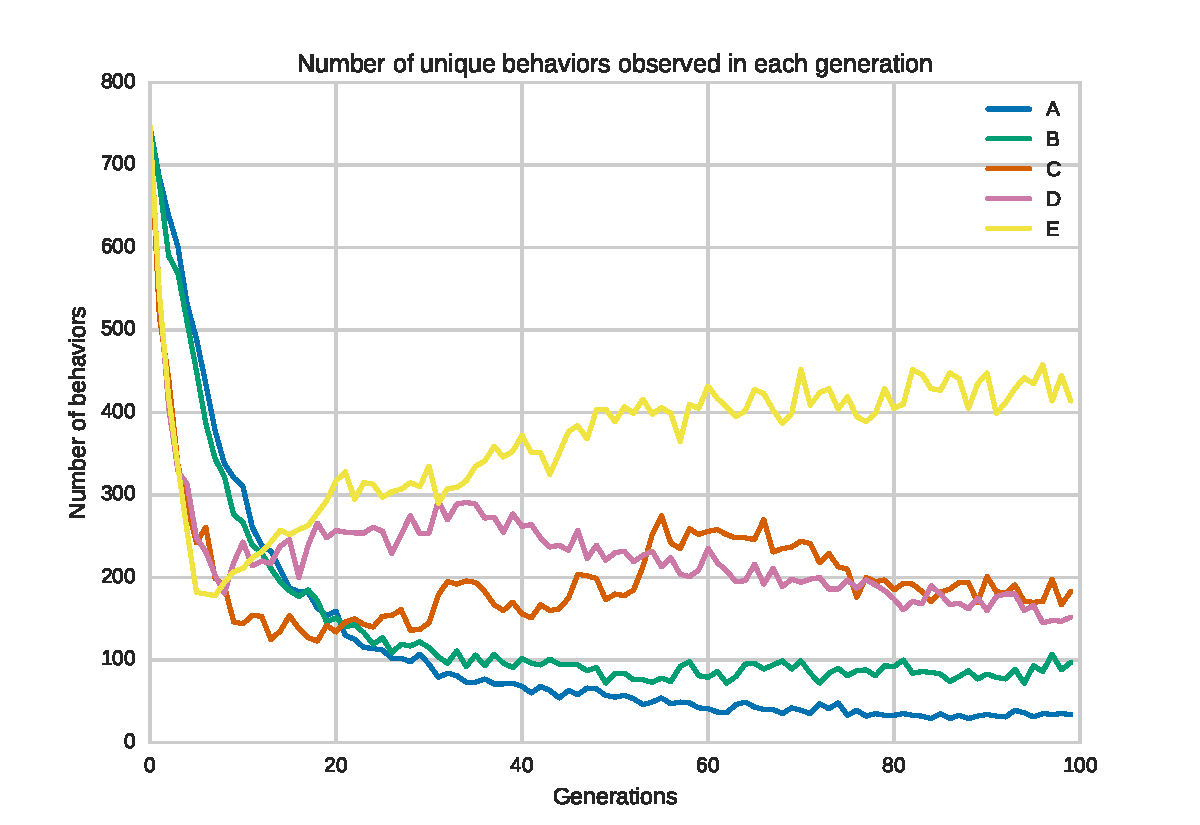
\includegraphics[width=\columnwidth]{fig/unique_behaviors}
\caption{TODO}
\end{figure}
